\documentclass[10.5pt,scale=1.0,t,aspectratio=169,hyperref={pdfpagelabels=false}]{beamer}


\usepackage{lipsum}
\usepackage{color}
\usepackage{amsfonts}
\usepackage{amsmath,mathtools}
\usepackage{mathrsfs}
\usepackage{array}
\usepackage{algorithm}
\usepackage{hyperref}
\usepackage[spanish,es-nodecimaldot]{babel}
\usepackage[utf8]{inputenc}
\usepackage{graphicx}
\usepackage{multicol}
\usepackage{multirow}
\usepackage{enumitem}
\usepackage[document]{ragged2e}
\usepackage[absolute,overlay]{textpos}
\textblockorigin{0mm}{0mm} 
\usefonttheme[onlymath]{serif}
\usepackage{verbatim}
\usepackage{cite}
\usepackage{multicol}




\newenvironment{conditions}[1][where:]
{#1 \begin{tabular}[t]{>{$}l<{$} @{${}={}$} l}}
	{\end{tabular}\\[\belowdisplayskip]}


\newcolumntype{L}{>{$}l<{$}} % math-mode version of "l" column type


\newcounter{saveenumi}
\newcommand{\seti}{\setcounter{saveenumi}{\value{enumi}}}
\newcommand{\conti}{\setcounter{enumi}{\value{saveenumi}}}

\setbeamertemplate{bibliography item}{\insertbiblabel}


\hypersetup{colorlinks=true,
	linkcolor=blue,
	linktoc=all,				
	citecolor=blue,
	urlcolor=red,
	pdftitle={ELECTRONICA DIGITAL II},
	pdfauthor={Santiago Rúa Pérez},
	pdfcreator={Santiago Rúa Pérez}}


\definecolor{GreenDark}{rgb}{0.0, 0.60, 0.0}
\definecolor{RedDark}{rgb}{183, 0.0, 0.0}
\definecolor{BlueDark}{rgb}{0.0, 0.0, 167}
\definecolor{BlueLight}{rgb}{0.2, 0.451, 0.517}


\graphicspath{{imag/}}

\newcommand{\Ho}{$H_{0}$}
\newcommand{\Ha}{$H_{a}$}
\newcommand{\Nota}{{\bf Nota: }}
\newcolumntype{P}[1]{>{\centering\arraybackslash}p{#1}}
\newcolumntype{M}[1]{>{\centering\arraybackslash}m{#1}}

\newcommand{\less}{<}
\newcommand{\greater}{>}


\setlength{\parindent}{1em}
\setlength{\parskip}{.6em}
\renewcommand{\baselinestretch}{.9}

%%%%    C environment    ---------------- %%%%%%%%%%%%%%%.
\usepackage{listings}
\usepackage{xcolor}
\definecolor{mGreen}{rgb}{0,0.6,0}
\definecolor{mGray}{rgb}{0.5,0.5,0.5}
\definecolor{mPurple}{rgb}{0.58,0,0.82}
\definecolor{backgroundColour}{rgb}{0.95,0.95,0.92}

\lstdefinestyle{CStyle}{
	backgroundcolor=\color{backgroundColour},   
	commentstyle=\color{mGreen},
	keywordstyle=\color{magenta},
	numberstyle=\tiny\color{mGray},
	stringstyle=\color{mPurple},
	basicstyle=\scriptsize,
	breakatwhitespace=false,         
	breaklines=true,                 
	captionpos=b,                    
	keepspaces=true,                 
	numbers=left,                    
	numbersep=5pt,                  
	showspaces=false,                
	showstringspaces=false,
	showtabs=false,                  
	tabsize=2,
	language=C
}
%%--------------------------------------------------------------------------


\title{Electrónica Digital II}   
\author{Santiago Rúa Pérez, PhD.} 
\date{\today} 

\setlength{\TPHorizModule}{\textwidth}
\setlength{\TPVertModule}{\textwidth}

\newcommand{\btVFill}{\vskip0pt plus 1filll}


\setbeamertemplate{sidebar right}{}
\setbeamertemplate{footline}
{
	\leavevmode%
	\hbox{%
		\begin{beamercolorbox}[wd=.333333\paperwidth,ht=2.25ex,dp=1ex,center]{author in head/foot}%
			\usebeamerfont{author in head/foot}\insertshortauthor
		\end{beamercolorbox}%
		\begin{beamercolorbox}[wd=.333333\paperwidth,ht=2.25ex,dp=1ex,center]{title in head/foot}%
			\usebeamerfont{title in head/foot}\insertshorttitle
	\end{beamercolorbox}}%
	\vskip0pt%
}
\makeatother

\begin{document}
	%%%%%%%%%%%%%%%%%% FRAME %%%%%%%%%%%%%%%%%%%%%%%%%%
	\begin{frame}
		\titlepage
	\end{frame}
	%%%%%%%%%%%%%%%%% FRAME START %%%%%%%%%%%%%%%%%%%%%%%%%%
	\frame{
		%\frametitle{}
		\begin{center}
			\LARGE \textcolor{blue}{CONCURRENCIA BÁSICA}
		\end{center}
		
	}
	
	%%%%%%%%%%%%%%%%% FRAME %%%%%%%%%%%%%%%%%%%%%%%%%%

%%%%%%%%%%%%%%%%% FRAME %%%%%%%%%%%%%%%%%%%%%%%%%%
\begin{frame}
\frametitle{Objetivos}
\begin{itemize}
\item Entender como realizar un programa modular.
\item Medira la sensibilidad de un sistema o software.
\item Comprender la sobrecarga de la CPU.
\item Trabajar con interrupciones y eventos. 
\end{itemize}
\end{frame}
%%%%%%%%%%%%%%%%% FRAME %%%%%%%%%%%%%%%%%%%%%%%%%%
\begin{frame}
	\frametitle{Reto de planificación}
	Cómo compartir los recursos de la CPU entre diferentes actividades o tareas que tiene el software?
	\begin{itemize}
		\item Típicamente un sistema embebido tiene múltiples tareas que debe administrar.
		\begin{itemize}
			\item Algunas son realizadas por los periféricos, otras por software en la CPU.
		\end{itemize}  
		\item Cada actividad tiene requerimientos de tiempo, y algunos son más críticos que otros. 
		\begin{itemize}
			\item Ejemplos: lecturas de pulsadores, escanear LEDs.
		\end{itemize} 
		\item Se desea que solo una CPU parezca que puede hacer muchas cosas al tiempo de forma concurrente. 
		\begin{itemize}
			\item Inclusive con procesadores multinúcleo, se tiene mas tareas que procesadores. 
		\end{itemize}
		\item Como compartir la CPU entre diferentes tareas? Como simulamos concurrencia entre las diferentes actividades? \textbf{Como hacemos planificación de tareas}?
	\end{itemize}
\end{frame}
%%%%%%%%%%%%%%%%% FRAME %%%%%%%%%%%%%%%%%%%%%%%%%%
\begin{frame}
	\frametitle{Roadmap}
	\begin{itemize}
		\item Modularidad: que tanto el programa está estructurado en pequeñas porciones funcionales.
		\item Respuesta: medir que tan rápido el sistema responde ante un evento.
		\item Sobrecarga de la CPU: cuanto tiempo se demora la CPU ejecutando instrucciones fuera de las principales. 
	\end{itemize}	
	\begin{figure}
		\centering
		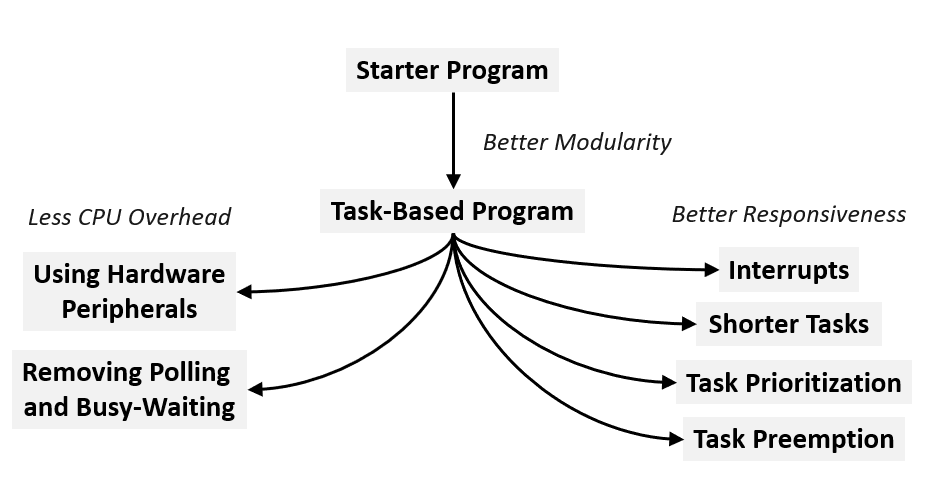
\includegraphics[scale=0.35]{01_SchedullingRoadmap}
	\end{figure}
\end{frame}

%%%%%%%%%%%%%%%%% FRAME %%%%%%%%%%%%%%%%%%%%%%%%%%
\begin{frame}
	\frametitle{Problema a resolver}
	Se tiene un sistema con dos pulsadores y un LED RGB. 
	\begin{itemize}
		\item Cuando el suiche 1 no se presiona, el sistema muestra una secuencia de forma repetitiva (R-G-B).
		\item Cuando se presiona 1, comienza a parpadear en blanco (todos prendidos), hasta que se libera
		\item Mientras se mantenga presionado 2, es más rápido el parpadeo y la secuencia RGB.
	\end{itemize}
	\begin{figure}
		\centering
		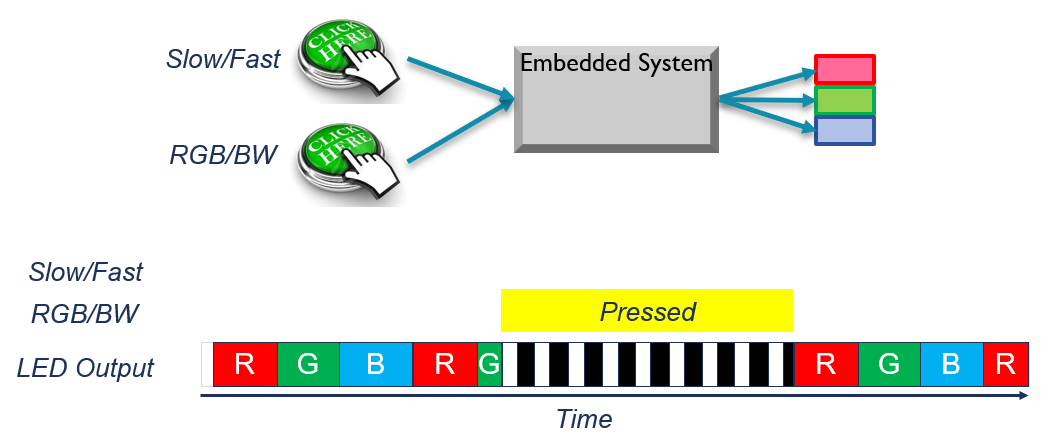
\includegraphics[scale=0.35]{02_ParpadeoEjemplo}
	\end{figure}
\end{frame}

%%%%%%%%%%%%%%%%% FRAME %%%%%%%%%%%%%%%%%%%%%%%%%%
\begin{frame}
	\frametitle{Planificación ideal - Manejado por eventos}
	\begin{figure}
		\centering
		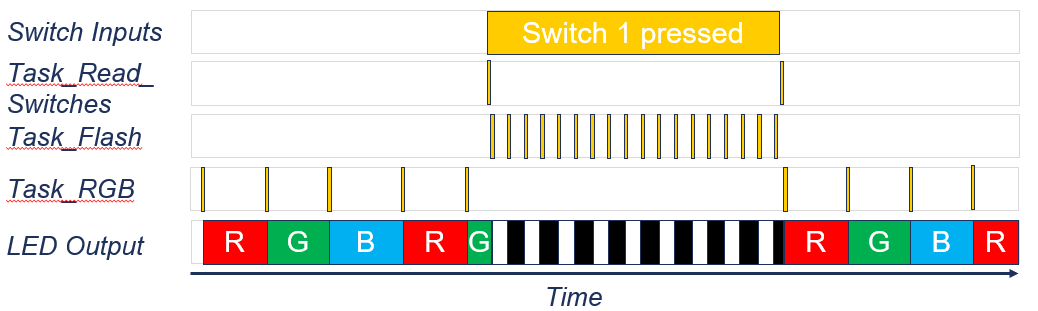
\includegraphics[scale=0.5]{03_IdealSchedulling}
	\end{figure}

\begin{itemize}
	\item Note que la ejecución de cada tarea consume poco tiempo dentro del diagrama.
	\item Inmediatamente se presiona el suiche el estado del Led cambia y solo tarda lo que demora la tarea de lectura y de parpadeo. 
\end{itemize}
\end{frame}
%%%%%%%%%%%%%%%%% FRAME %%%%%%%%%%%%%%%%%%%%%%%%%%
\begin{frame}[fragile]
	\frametitle{Solución 1}
	\begin{multicols}{2}
\begin{lstlisting}[style=CStyle]
#define W_DELAY_SLOW 400
#define W_DELAY_FAST 200
#define RGB_DELAY_SLOW 4000
#define RGB_DELAY_FAST 1000

void Flasher(void) {
	uint32_t w_delay = W_DELAY_SLOW;
	uint32_t RGB_delay = RGB_DELAY_SLOW;
	
	Init_GPIO_RGB();
	Init_GPIO_Switches();
	while (1) {
		if (SWITCH_PRESSED(SW1_POS)) {	// flash white
			Control_RGB_LEDs(1, 1, 1);
			Delay(w_delay);
			Control_RGB_LEDs(0, 0, 0);
			Delay(w_delay);
		} else {										// sequence R, G, B
			Control_RGB_LEDs(1, 0, 0);
			Delay(RGB_delay);
			Control_RGB_LEDs(0, 1, 0);
			Delay(RGB_delay);
			Control_RGB_LEDs(0, 0, 1);
			Delay(RGB_delay);
		}
		if (SWITCH_PRESSED(SW2_POS)) {
			w_delay = W_DELAY_FAST;
			RGB_delay = RGB_DELAY_FAST;
		} else {
			w_delay = W_DELAY_SLOW;
			RGB_delay = RGB_DELAY_SLOW;
		}
	}
}
\end{lstlisting}
	\end{multicols}
Qué pasa cuando se presiona el suiche 1 cuando esta en verde el led?
\end{frame}
%%%%%%%%%%%%%%%%% FRAME %%%%%%%%%%%%%%%%%%%%%%%%%%
\begin{frame}
	\frametitle{Análisis - Solución 1}
	\begin{figure}
		\centering
		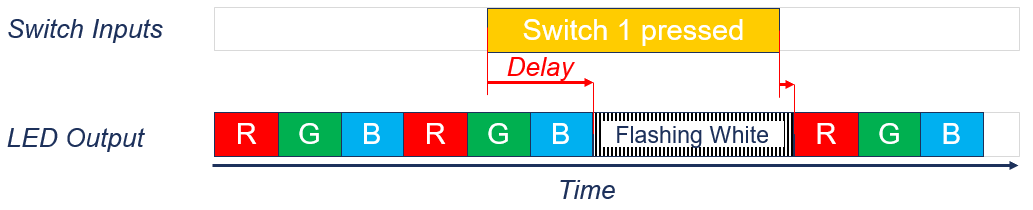
\includegraphics[scale=0.45]{04_TimingSolution1}
	\end{figure}
\begin{itemize}
	\item Considere el programa realizado.
	\item Problemas:
	\begin{itemize}
		\item Tiene mantener presionado el interruptor hasta que el programa lo sondea, puede haber una gran demora.
		\item Algunas veces que se presiona el interruptor pueden ignorarse.
	\end{itemize}
	\item El programa solo lee los interruptores por cada ciclo del LED.
	\item El ciclo de escaneo del LED puede tomar mayor tiempo.
\end{itemize}
\end{frame}
%%%%%%%%%%%%%%%%% FRAME %%%%%%%%%%%%%%%%%%%%%%%%%%
\begin{frame}
	\frametitle{Creando y usando tareas}
	Una estructura buena de codificación simplifica el desarrollo
	\begin{itemize}
		\item Tareas: código que desarrolla una actividad, o conjunto de actividades.
		\begin{itemize}
			\item Parpadear leds.
			\item Leer interruptores.
		\end{itemize}
		\item Simplifica el desarrollo.
		\begin{itemize}
			\item Agrupar por funcionalidades similares.
			\item Separar funcionalidades diferentes.
			\item Mejora el debug, mantenimiento y desarrollo. 
		\end{itemize}
		\item Cada tarea es llamada desde otra tarea o función principal.
		\begin{itemize}
			\item La tarea principal puede llamar a otras funciones que necesite. 
		\end{itemize}
	\end{itemize}
\end{frame}
%%%%%%%%%%%%%%%%% FRAME %%%%%%%%%%%%%%%%%%%%%%%%%%
\begin{frame}
	\frametitle{Solución 2}
	\begin{columns}
		\column{0.5\linewidth}
		\begin{itemize}
			\item Se utilizan variables globales para compartir información. 
			\item Las flechas indican quien modifica y lee las variables globales. 
			\item Este tipo de esquema se llama multitarea cooperativa, si una tarea se demora mucho entonces las demás les toca esperar. 
		\end{itemize}
		\column{0.5\linewidth}
		\begin{figure}
			\centering
			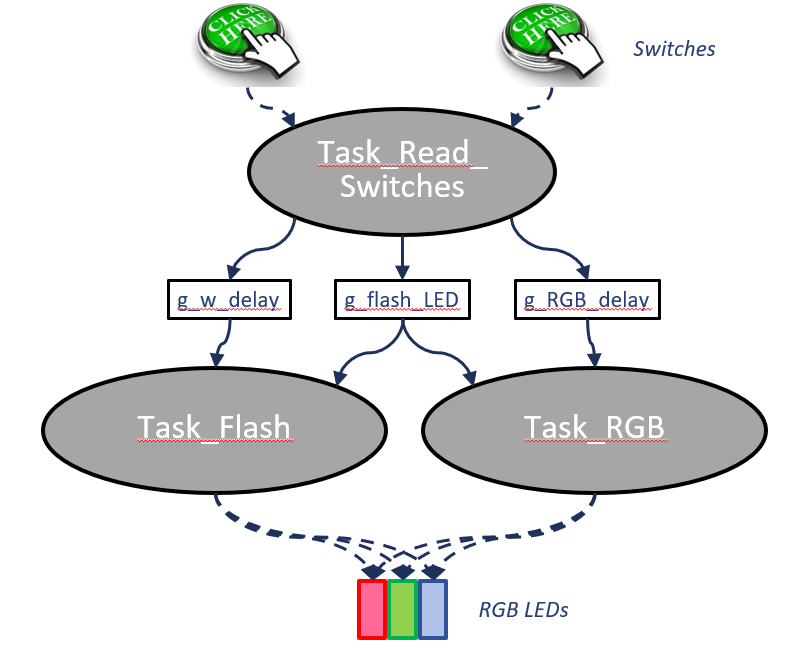
\includegraphics[scale=0.35]{05_TaskSolution2}
		\end{figure}
	\end{columns}
\end{frame}
%%%%%%%%%%%%%%%%% FRAME %%%%%%%%%%%%%%%%%%%%%%%%%%
\begin{frame}[fragile]
	\frametitle{Solución 2 - Código}
	
	Tarea de lectura de los suiches
	
	\begin{lstlisting}[style=CStyle]
volatile uint8_t g_flash_LED = 0;
volatile uint32_t g_w_delay = W_DELAY_SLOW;
volatile uint32_t g_RGB_delay = RGB_DELAY_SLOW;

void Task_Read_Switches(void) {
	if (SWITCH_PRESSED(SW1_POS)) {
		g_flash_LED = 1; // flash white
	} else {
		g_flash_LED = 0; // RGB sequence
	}
	if (SWITCH_PRESSED(SW2_POS)) { 
		g_w_delay = W_DELAY_FAST;
		g_RGB_delay = RGB_DELAY_FAST;
	} else {
		g_w_delay = W_DELAY_SLOW;
		g_RGB_delay = RGB_DELAY_SLOW;
	}
}
	\end{lstlisting}
\end{frame}
%%%%%%%%%%%%%%%%% FRAME %%%%%%%%%%%%%%%%%%%%%%%%%%
\begin{frame}[fragile]
	\frametitle{Solución 2 - Código}
	
	Tarea de parpadear el led y secuencia RGB
	\begin{lstlisting}[style=CStyle]
void Task_Flash(void) {
	if (g_flash_LED == 1) { // Only run task when in flash mode
		Control_RGB_LEDs(1, 1, 1);
		Delay(g_w_delay);
		Control_RGB_LEDs(0, 0, 0);
		Delay(g_w_delay);
	}
}
void Task_RGB(void) {
	if (g_flash_LED == 0) { //only run task when NOT in flash mode
		Control_RGB_LEDs(1, 0, 0);
		Delay(g_RGB_delay);
		Control_RGB_LEDs(0, 1, 0);
		Delay(g_RGB_delay);
		Control_RGB_LEDs(0, 0, 1);
		Delay(g_RGB_delay);
	}
}
	\end{lstlisting}
\end{frame}
%%%%%%%%%%%%%%%%% FRAME %%%%%%%%%%%%%%%%%%%%%%%%%%
\begin{frame}[fragile]
	\frametitle{Solución 2 - Código}
	
	Programa principal o tarea principal
	\begin{lstlisting}[style=CStyle]
void Flasher(void) {
	Init_GPIO_RGB();
	Init_GPIO_Switches();
	while (1) {
		Task_Read_Switches();
		Task_Flash();
		Task_RGB();
	}
}
	\end{lstlisting}

Cada tarea es llamada de forma secuencial, por lo que la ejecución dependerá de la más lenta. 
\end{frame}
%%%%%%%%%%%%%%%%% FRAME %%%%%%%%%%%%%%%%%%%%%%%%%%
\begin{frame}
	\frametitle{Análisis - Solución 2}
	\begin{figure}
		\centering
		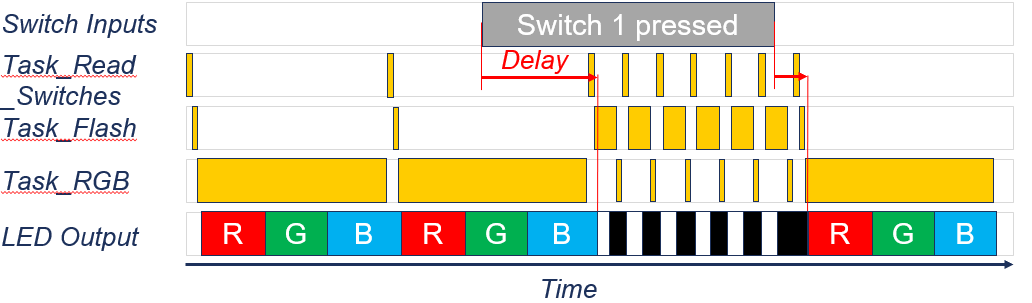
\includegraphics[scale=0.4]{06_TimingSolution2}
	\end{figure}
	\begin{itemize}
		\item Flasher es un planificador de tareas (\textbf{task scheduler}), el cual hace un llamado a cada tarea. Cada tarea se ejecuta y devuelve el control al planificador.
		\item Máximo retardo ocurre cuando se presiona el interruptor justo cuando inicia la secuencia RGB. 
		\item Cada tarea se ejecuta después 
	\end{itemize}
\end{frame}
%%%%%%%%%%%%%%%%% FRAME %%%%%%%%%%%%%%%%%%%%%%%%%%
\begin{frame}
	\frametitle{Considerar retrasos entre tareas}
	\begin{figure}
		\centering
		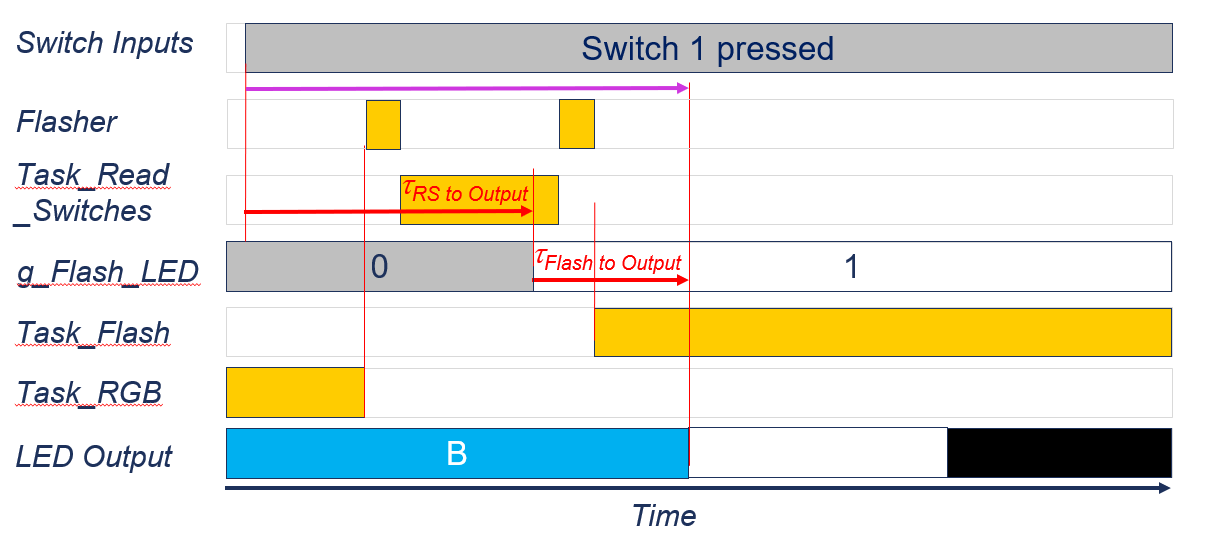
\includegraphics[scale=0.4]{07_TimingDelay2}
	\end{figure}
	\begin{itemize}
		\item La tarea de lectura de interruptores cambia la salida despues de $\tau_{RS}$.
		\item La tarea de parpadear cambia el led despues del retraso $\tau_{Flash}$
		\item Se puede mejorar utilizando interrupciones en vez de polling. 
	\end{itemize}
\end{frame}
%%%%%%%%%%%%%%%%% FRAME %%%%%%%%%%%%%%%%%%%%%%%%%%
\begin{frame}
	\frametitle{Conceptos de interrupciones}
	\begin{columns}
		\column{0.5\linewidth}
		\begin{itemize}
			\item Interrupción
			\begin{itemize}
				\item Señal que indica que un evento particular pasó.
			\end{itemize}
			\item Comportamiento del sistema.
			\begin{itemize}
				\item CPU está ejecutando programas.
				\item La interrupción fuerza al sistema a parar y correr una función especial (Interrupt Service Routine ISR), el cual atiende el evento. 
				\item Después de que finaliza, el control vuelve a la CPU.
			\end{itemize}
			\item Nunca se llamada a una función ISR desde el código.
		\end{itemize}
		\column{0.5\linewidth}
		\begin{figure}
			\centering
			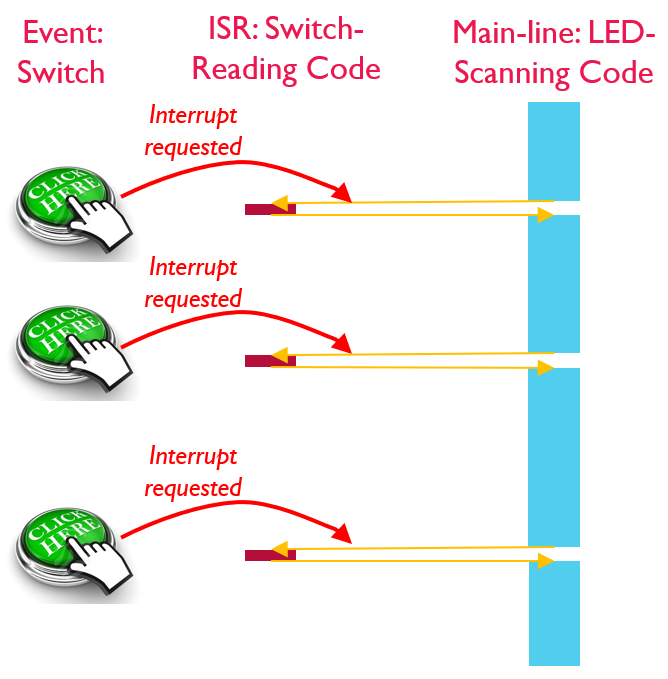
\includegraphics[scale=0.4]{08_ISRDiagram}
		\end{figure}
	\end{columns}
\end{frame}
%%%%%%%%%%%%%%%%% FRAME %%%%%%%%%%%%%%%%%%%%%%%%%%
\begin{frame}
	\frametitle{Solución 3}
	\begin{columns}
		\column{0.5\linewidth}
		\begin{itemize}
			\item Utilizar rutina de servicio de interrupción para los suiches.
			\item Comunicarse a través de variables globales.  
		\end{itemize}
		\column{0.5\linewidth}
		\begin{figure}
			\centering
			\includegraphics[scale=0.3]{09_solutionV3}
		\end{figure}
	\end{columns}
\end{frame}
%%%%%%%%%%%%%%%%% FRAME %%%%%%%%%%%%%%%%%%%%%%%%%%
\begin{frame}[fragile]
	\frametitle{Solución 3 - Código}

	\begin{lstlisting}[style=CStyle]
volatile uint8_t g_flash_LED = 0;
volatile uint32_t g_w_delay = W_DELAY_SLOW;
volatile uint32_t g_RGB_delay = RGB_DELAY_SLOW;

void PORTD_IRQHandler(void){
	if ((PORTD->ISRF & MASK(SW1_POS))) {
		if (SWITCH_PRESSED(SW1_POS)) {
			g_flash_LED = 1;					// 
		} else {
			g_flash_LED = 0;					// RGB 
		}
	}
	if ((PORTD->ISRF & MASK(SW2_POS))) {
		if (SWITCH_PRESSED(SW2_POS)) {	// Short delays
			g_w_delay = W_DELAY_FAST;
			g_RGB_delay = RGB_DELAY_FAST;
		} else {									
			g_w_delay = W_DELAY_SLOW;
			g_RGB_delay = RGB_DELAY_SLOW;
		}
	}
	PORTD->ISFR = 0XFFFFFFFF;
}
	\end{lstlisting}
\end{frame}
%%%%%%%%%%%%%%%%% FRAME %%%%%%%%%%%%%%%%%%%%%%%%%%
\begin{frame}
	\frametitle{Análisis - Solución 3}
	\begin{figure}
		\centering
		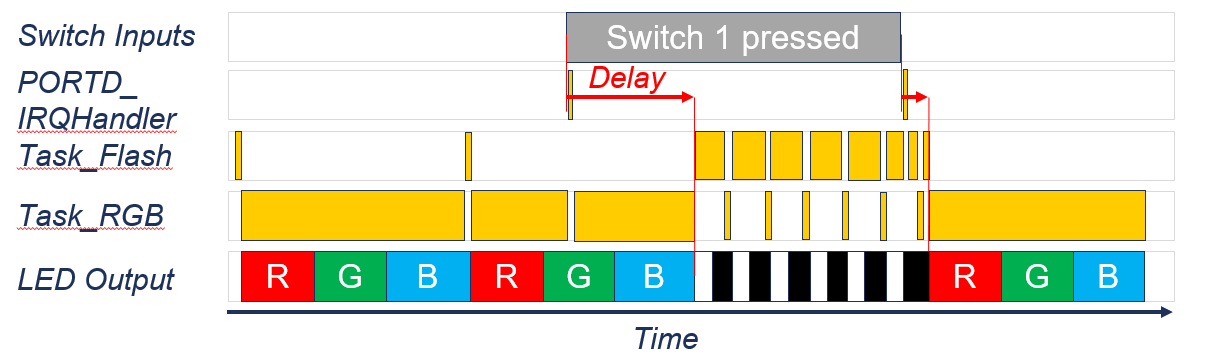
\includegraphics[scale=0.4]{10_TimingSolution3}
	\end{figure}
	\begin{itemize}
		\item Mejoramiento limitado del ISR, ya que la tarea de RGB sigue su ejecución.
		\begin{itemize}
			\item La tarea de RGB pone limitantes.
			\item Ejemplo de un sistema no preventivo (non-preemptive): las tareas no puede apropiarse de los recursos mientras se ejecuta otra.
		\end{itemize}
	\end{itemize}
\end{frame}
%%%%%%%%%%%%%%%%% FRAME %%%%%%%%%%%%%%%%%%%%%%%%%%
\begin{frame}
	\frametitle{Como podemos mejorar tiempo de respuesta?}
\begin{columns}
	\column{0.5\linewidth}
	\begin{itemize}
		\item Adicionar mas test dentro de las tareas? 
		\begin{itemize}
			\item Posibilita que la tarea termine antes.
		\end{itemize}
		\item Mala idea
		\begin{itemize}
			\item Mezcla diferente tareas para el planificador.
			\item Código extra de ejecución.
			\item Dificil de mantener en el tiempo. 
		\end{itemize}
		\item Modificar la función de retraso para terminar antes? Código spaghetti
	\end{itemize}
	\column{0.5\linewidth}
	\begin{figure}
		\centering
		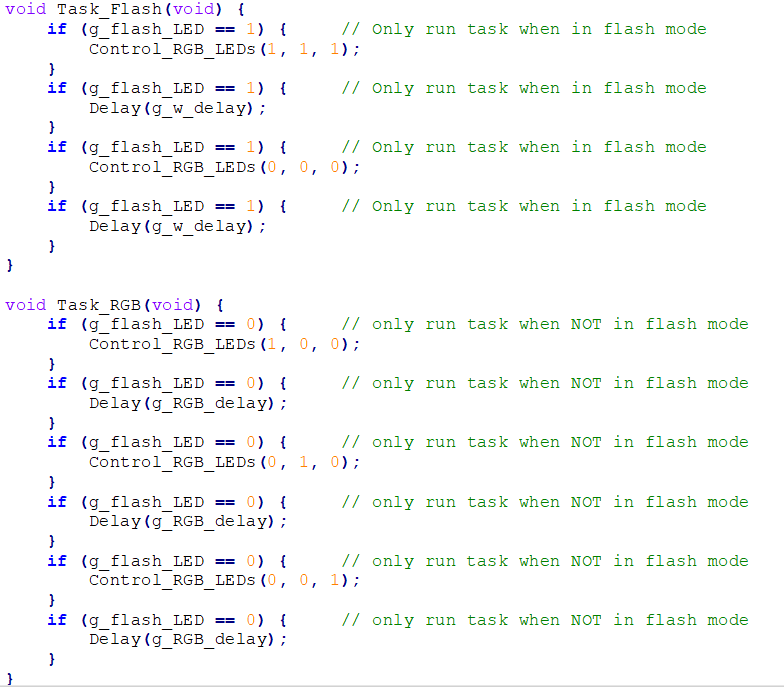
\includegraphics[scale=0.4]{11_MoreTest}
	\end{figure}
\end{columns}
	
\end{frame}
%%%%%%%%%%%%%%%%% FRAME %%%%%%%%%%%%%%%%%%%%%%%%%%
\begin{frame}
	\frametitle{Como podemos mejorar tiempo de respuesta?}
	Mover más código al ISR?
	\begin{figure}
		\centering
		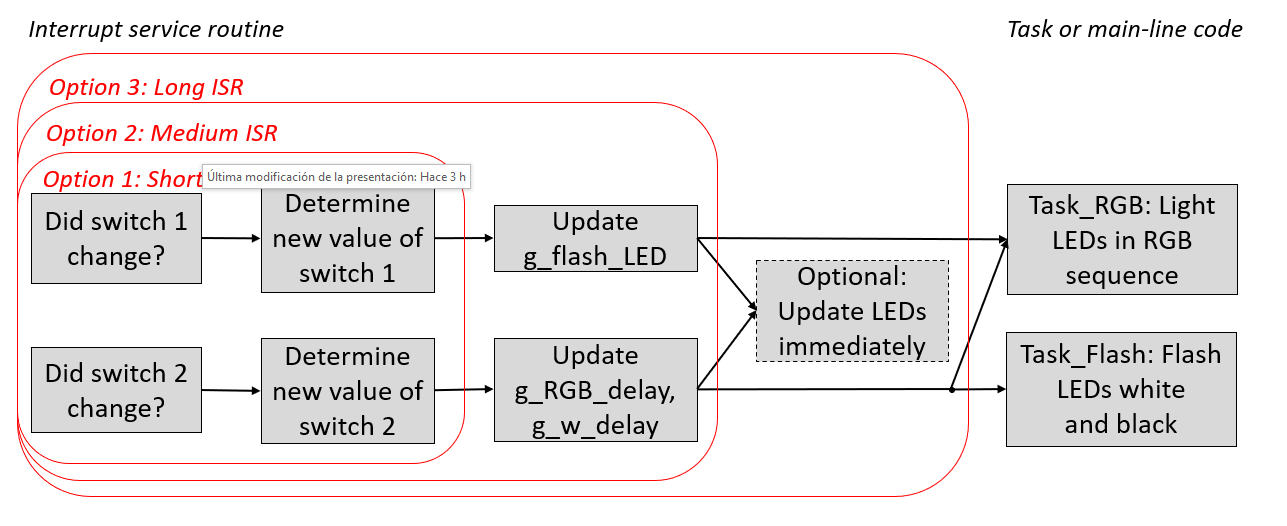
\includegraphics[scale=0.4]{12_MoreISR}
	\end{figure}
	\textbf{Solución}: Utilizar máquinas de estado finito. 
\end{frame}
%%%%%%%%%%%%%%%%% FRAME %%%%%%%%%%%%%%%%%%%%%%%%%%
\begin{frame}
	\frametitle{Reducir tiempo de respuesta con FSM}
	\begin{columns}
		\column{0.5\linewidth}
		\begin{itemize}
			\item Reescribir cada tarea para returno el control al planificador cuando antes.
			\item Cada llamado ejecuta un estado al tiempo. 
			\item \textbf{Objetivo}: reducir tiempos largos de consumo de una tarea.
			\item Utilizar un case por cada estado. 
		\end{itemize}
		\column{0.5\linewidth}
		\begin{figure}
			\centering
			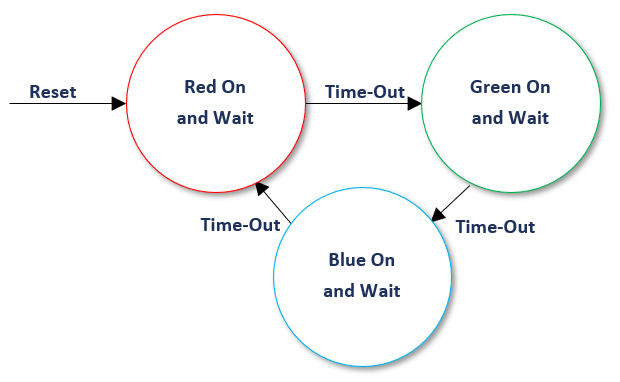
\includegraphics[scale=0.4]{13_FSMExample}
		\end{figure}
	\end{columns}
\end{frame}
%%%%%%%%%%%%%%%%% FRAME %%%%%%%%%%%%%%%%%%%%%%%%%%
\begin{frame}
	\frametitle{Solución 4 - FSM}
	\begin{figure}
		\centering
		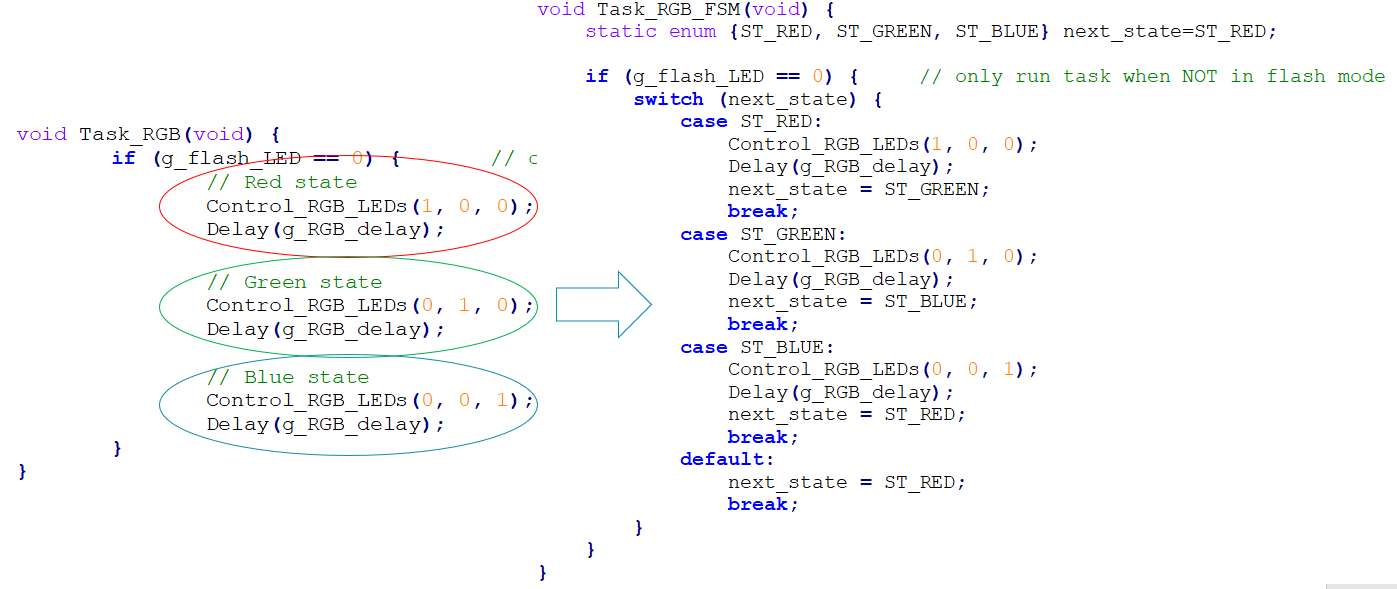
\includegraphics[scale=0.4]{14_TaskToFSM}
	\end{figure}
\end{frame}
%%%%%%%%%%%%%%%%% FRAME %%%%%%%%%%%%%%%%%%%%%%%%%%
\begin{frame}
	\frametitle{Solución 4 - FSM}
	\begin{figure}
		\centering
		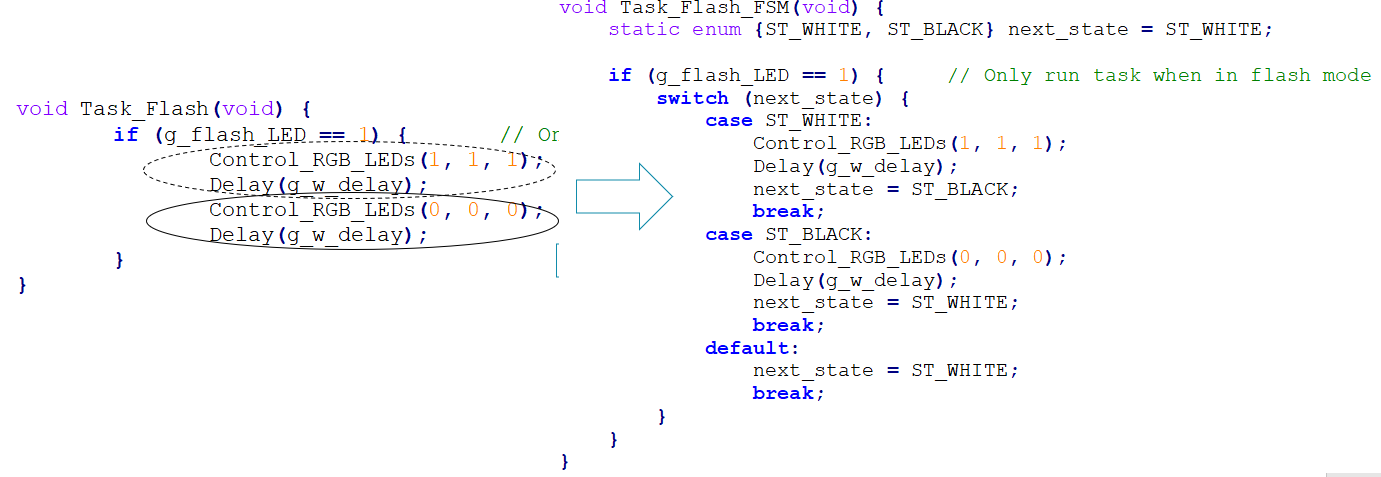
\includegraphics[scale=0.4]{15_TaskFlashFSM}
	\end{figure}
\end{frame}
%%%%%%%%%%%%%%%%% FRAME %%%%%%%%%%%%%%%%%%%%%%%%%%
\begin{frame}
	\frametitle{Análisis - Solución 4}
	\begin{figure}
		\centering
		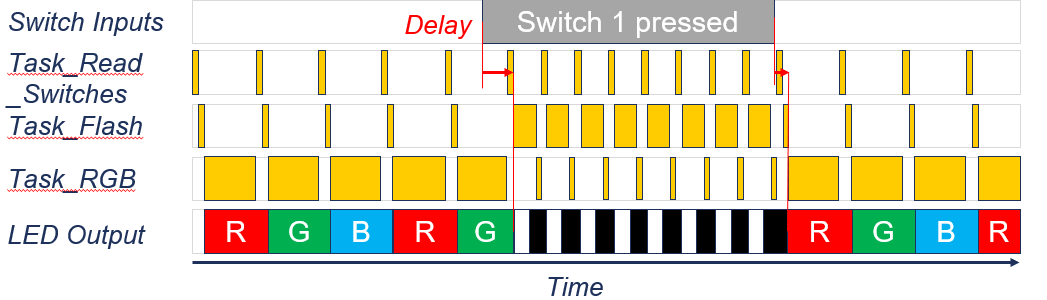
\includegraphics[scale=0.4]{16_TimingSolution4}
	\end{figure}
	\begin{itemize}
		\item Máximo retardo después de presionar el LED, aprox 1/3 mas corto. 
		\item \textbf{Nota}: se esta realizando polling de nuevo para permitir comparación directa. 
		\item Un poco de sobrecarga con FSM, pero aceptable.
		\item Software organizado en tareas. 
	\end{itemize}
\end{frame}
%%%%%%%%%%%%%%%%% FRAME %%%%%%%%%%%%%%%%%%%%%%%%%%
\begin{frame}
	\frametitle{Usar hardware para conservar tiempo de CPU - Solución 5}
	\begin{columns}
		\column{0.5\linewidth}
		\begin{itemize}
			\item La función de retardo usa un loop que retarda el programa. 
			\item Mejoría:
			\begin{itemize}
				\item Usar timer por hardware para llevar el tiempo.
				\item Software puede consultar el timer para determinar si ya paso el tiempo.
				\item Periódicamente preguntar por el timer. 
			\end{itemize}
		\end{itemize}
		\column{0.5\linewidth}
		\begin{figure}
			\centering
			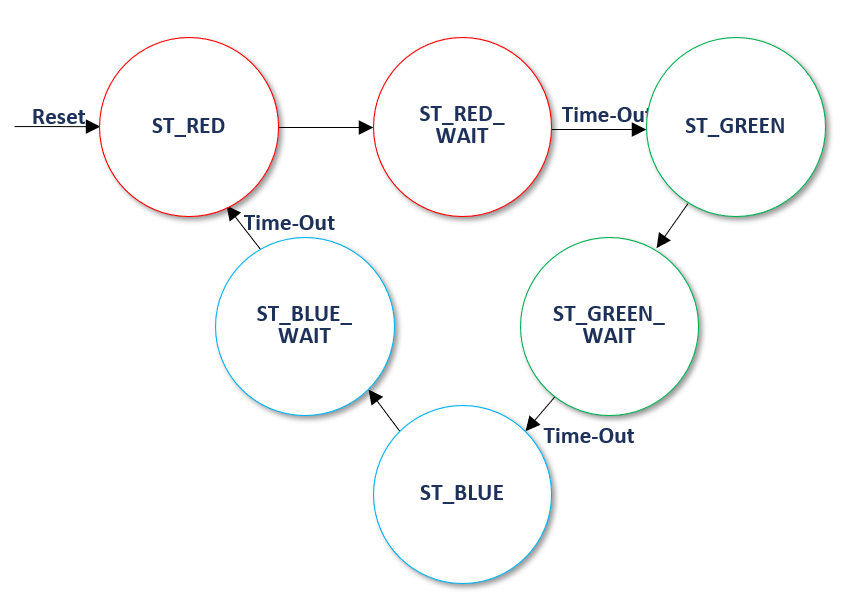
\includegraphics[scale=0.3]{17_FSMHardware}
		\end{figure}
	\end{columns}
\end{frame}
%%%%%%%%%%%%%%%%% FRAME %%%%%%%%%%%%%%%%%%%%%%%%%%
\begin{frame}
	\frametitle{Análisis - Solución 5}
	\begin{figure}
		\centering
		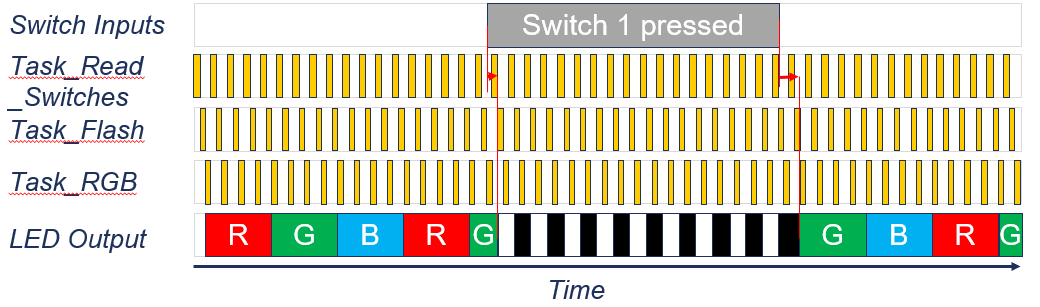
\includegraphics[scale=0.5]{17_TimingSolution5}
	\end{figure}
	\begin{itemize}
		\item Todos los estados se ejecutan y retornan rápidamente el control al planificador.
		\item El planificador da una vuelta más rápido. 
	\end{itemize}
\end{frame}
%%%%%%%%%%%%%%%%% FRAME %%%%%%%%%%%%%%%%%%%%%%%%%%
\begin{frame}
	\frametitle{Comparación Final}
	\begin{figure}
		\centering
		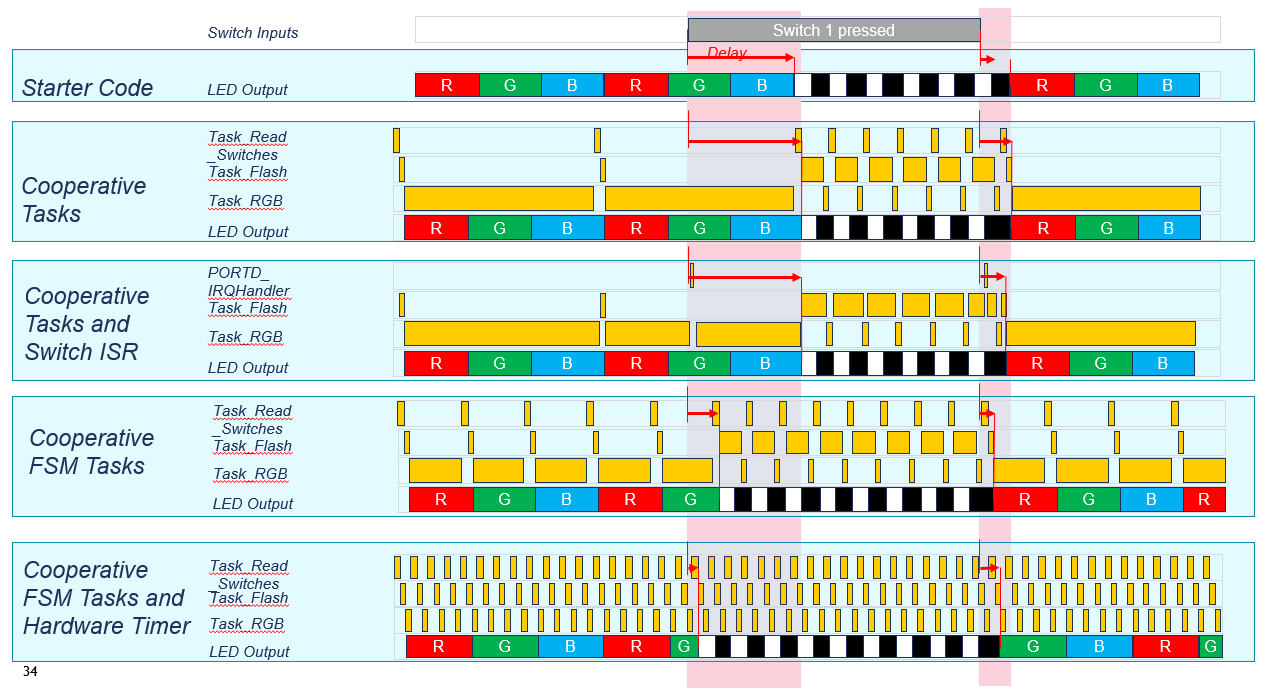
\includegraphics[scale=0.4]{18_Comparisson}
	\end{figure}	
\end{frame}
%%%%%%%%%%%%%%%%% FRAME %%%%%%%%%%%%%%%%%%%%%%%%%%
\begin{frame}
	\frametitle{Roadmap Final}
	\begin{columns}
		\column{0.5\linewidth}
		\begin{itemize}
			\item Agregue priorización a las tareas.
			\item Tareas con multipropósitos mas fácil de implementar. 
			\item Posibilita el control de tareas más fácil. 
		\end{itemize}
	\column{0.5\linewidth}
	\begin{figure}
		\centering
		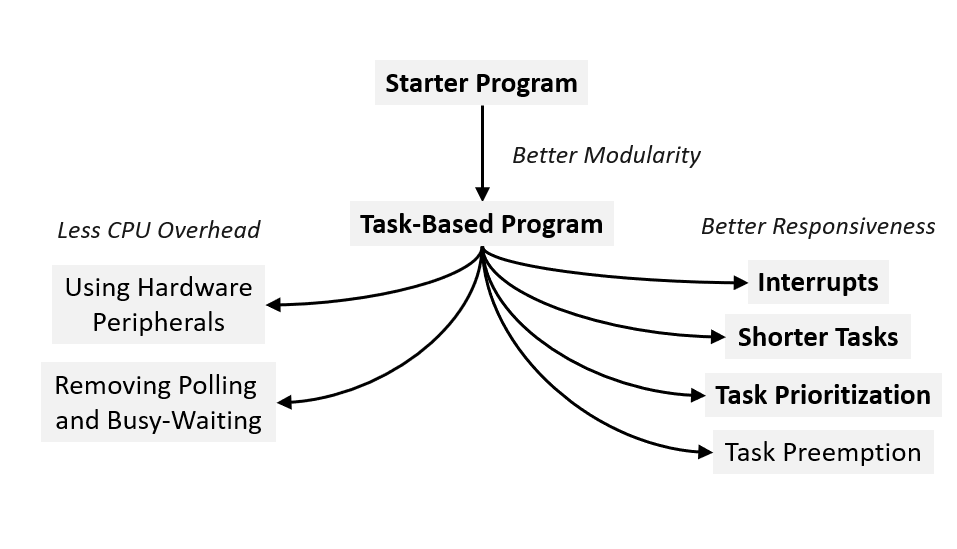
\includegraphics[scale=0.3]{19_RoadmapFinal}
	\end{figure}
\end{columns}
\end{frame}
%%%%%%%%%%%%%%%%% FRAME %%%%%%%%%%%%%%%%%%%%%%%%%%
\begin{frame}
\frametitle{Laboratorio 2 (15\%)}

Implementar el programa de la tarea RGB y pulsadores utilizando Máquinas de estado finito. 

\begin{itemize}
	\item Crear FSM para la secuenciación del led RGB.
	\item Crear FSM para el parpadeo blanco y negro del led.
\end{itemize}

\end{frame}
%%%%%%%%%%%%%%%%% FRAME %%%%%%%%%%%%%%%%%%%%%%%%%%
\frame{
\begin{center}
	\LARGE \textcolor{blue}{CONCURRENCIA BÁSICA}
\end{center}

\begin{center}
	\LARGE \textcolor{blue}{GRACIAS}
\end{center}
}

%%%%%%%%%%%%%%%%%%%%%%%%%%%%%%%%%%%%%%%%%%%%%%%%%%%%%%%%%%%%%%%%%%%%%%%%%%%%%%%%%%%%%%%%%%%%%%%%%%%%%%%%%%%%%



\end{document}

